\documentclass[
  shortnames]{jss}

\usepackage[utf8]{inputenc}

\providecommand{\tightlist}{%
  \setlength{\itemsep}{0pt}\setlength{\parskip}{0pt}}

\author{
Shannon K. Gallagher\\Biostatistics Research Branch\\
National Institute of Allergy\\
and Infectious Diseases \And Benjamin LeRoy\\Dept. of Statistics \& Data Science\\
Carnegie Mellon University
}
\title{Time invariant analysis of epidemics with \pkg{EpiCompare}}

\Plainauthor{Shannon K. Gallagher, Benjamin LeRoy}
\Plaintitle{Time invariant analysis of epidemics with EpiCompare}
\Shorttitle{\pkg{EpiCompare}}

\Abstract{
We present \pkg{EpiCompare}, an \proglang{R} package that suppliments
and enhance current infectious disease modeling analysis pipelines as
well as to encourage comparisons across these pipelines. A major
contribution of this work is the set of novel \textit{time-invariate}
tools for model and epidemic comparisons - including time-invariate
prediction bands. \pkg{EpiCompare} encorporates \proglang{R}'s
\textit{tidy} coding style to aid it rapid and easy use. This paper
provides an overview of both the tools in and intuition behind
\pkg{EpiCompare} and a thorough demonstrating of the tools through a
detailed example of a full data analysis pipeline.
}

\Keywords{keywords, not capitalized, \proglang{Java}}
\Plainkeywords{keywords, not capitalized, Java}

%% publication information
%% \Volume{50}
%% \Issue{9}
%% \Month{June}
%% \Year{2012}
%% \Submitdate{}
%% \Acceptdate{2012-06-04}

\Address{
    Shannon K. Gallagher\\
    Biostatistics Research Branch\\
  National Institute of Allergy\\
  and Infectious Diseases\\
    5603 Fishers Lane\\
Rockville, MD 20852\\
  E-mail: \email{shannon.gallagher@nih.gov}\\
  URL: \url{http://skgallagher.github.io}\\~\\
      Benjamin LeRoy\\
    Dept. of Statistics \& Data Science\\
  Carnegie Mellon University\\
    5000 Forbes Ave.\\
Pittsburgh, PA 15213\\
  E-mail: \email{bpleroy@andrew.cmu.edu}\\
  URL: \url{https://benjaminleroy.github.io/}\\~\\
  }


% Pandoc header
\usepackage{booktabs}
\usepackage{longtable}
\usepackage{array}
\usepackage{multirow}
\usepackage{wrapfig}
\usepackage{float}
\usepackage{xcolor}

\usepackage{amsmath}

\begin{document}

\newcommand{\shannon}[1]{\textcolor{orange}{#1}}
\newcommand{\ben}[1]{\textcolor{violet}{#1}}

\newtheorem{theorem}{Theorem}

\section[Intro]{Introduction}\label{sec:intro}

The recent (and currently on-going) COVID-19 global pandemic has
galvanized public interest in understanding more about infectious
disease modeling and has highlighted the usefulness of research in the
area of infectious disease epidemiology. Infectious disease models
typically attempt to do one or more of the following: 1) predict the
spread of current and future epidemics
\citep[e.g. flue prediction][]{Biggerstaff2016}, 2) analyze past and
current epidemics to increase scientific knowledge
\citep[e.g. historical measle outbreaks][]{Neal2004}, and 3) forecast or
project epidemic scenarios under pre-specified parameters
\citep[e.g. ...][]{}. The COVID-19 pandemic highlights how all three
goals are important both separately and taken as a whole. Infectious
diseases inflict enormous burdens on the world: millions of lives lost
and trillions of dollars spent yearly. Correctly analyzing and
addressing these issues aids in prevention and mitigation of future
outbreaks. \textcolor{orange}{really like this paragraph}

The current epidemic of COVID-19 also highlights that infectious disease
models are only one piece of the overall analysis pipeline. University
based resources like John Hopkin's and government numerical dashboards
(across all levels of government) during the COVID-19 epidemic remind us
that descriptive statistics and visualization can be a important first
step in the process (multiple \cite{}?).\}
\textcolor{orange}{add comment about NYT or something} Still, rightly
so, a large amount of theoretical work goes into modeling epidemics,
with different models focusing at the individual / agent level, network
structure or just aggregate flows (review paper \cite{}?). All placing
individuals / proportions of the populations into different states
(e.g.~suspectible, exposed, infected, recovered, etc.). With all these
models, review and comparison papers in the literature and through MIDAS
(Models of Infectious Disease Agent Study) Control Center helps the
individual practitioner decide the correct approach.
\textcolor{orange}{along with expertise from healthcare professionals...}

At the same time, analysis packages often only address a portion of the
analysis pipeline. Modeling tools often don't provide easy ways to
compare and assess their models on new data. Moreover, exploring and
modeling epidemics require transforming and \textit{tidying} data in
different ways. To fill these gaps, we present our our \proglang{R}
package \pkg{EpiCompare}. Our package's primary focus is to aid and
advance research in the area of comparison and assessment of epidemic \&
epidemiological models. In Figure \ref{fig:pipeline}, we illustrate the
data analysis pipeline of infectious diseases as 1) data pre-processing,
2) exploratory data analysis (EDA), 3) modeling and simulating, 4)
post-processing, and 5) comparison and assessment; where each previous
part of the pipeline influences the next. \pkg{EpiCompare} provides
tools to aids practitioners in all areas of this pipeline.

\begin{figure}[!ht]
    \centering
    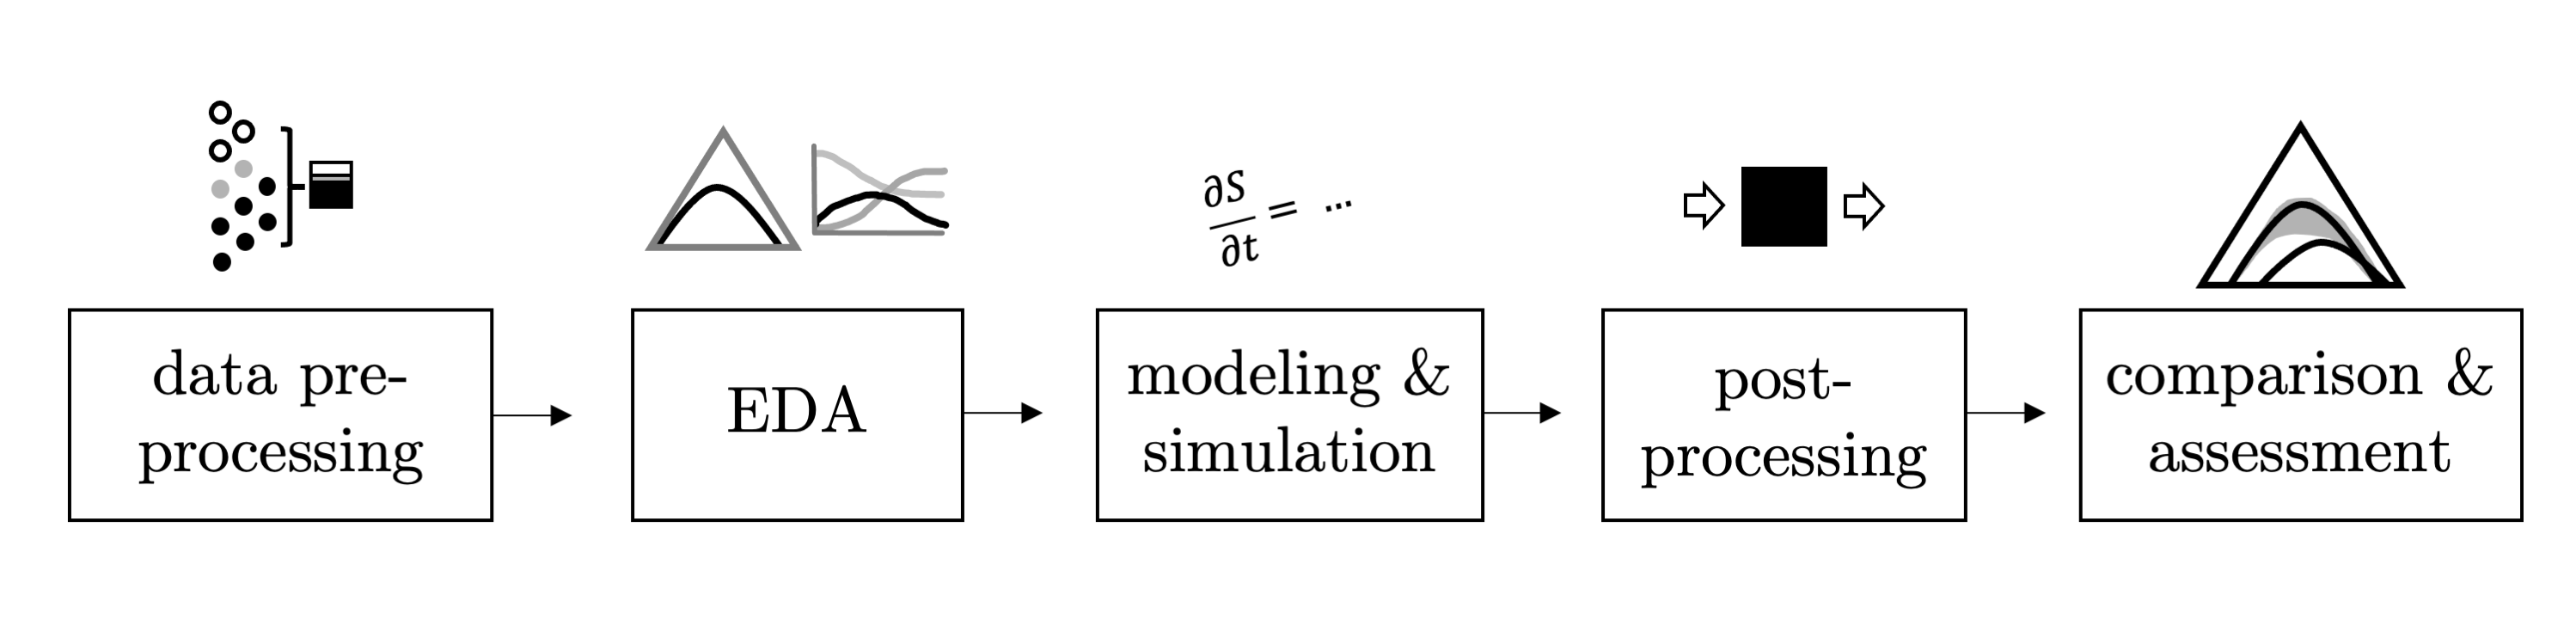
\includegraphics[width = 1\textwidth]{images/pipeline1.png}
    \caption{An idealized epidemiological data analysis pipeline.}
    \label{fig:pipeline}
\end{figure}

This package also emphasizes the value of approach epidemics in a
\textit{time-invariant} way, not constrained to things like a specific
time scale, or initial date of the first infection. Although epidemics
are by definition a process that evolves over time, epidemics, including
the recent COVID-19, often need to be compared in a time-invariant way
to understand the processes at play. Additionally, many tools to examine
the quantity of the population in each state along the infection process
(for example: quantity of suspectible vs infected vs recovered
individuals) don't always as intelligently capture the natural
connections between the proportion of individuals in these states. Tools
in \pkg{EpiCompare} attempt to give the user the ability to extend their
toolkit to evaluate epidemics to also include time-invariant approaches.
The goal of \pkg{EpiCompare} is not to supplant existing infectious
disease modeling tools and software but, rather, is a concerted effort
to create standard and fair comparisons among models developed for
disease outbreaks and outbreak data.
\textcolor{orange}{flesh out time invariance introduction to better explain to non-experts what we mean.  perhaps mention R0}

This paper is broken up into the following sections, section
\ref{sec:time-invariant} motivates and showcases tools of time-invariant
analysis, section \ref{sec:overview} presents an outline of how
\pkg{EpiCompare} aids a practitioner in every step of the pipeline and
section \ref{sec:tour} provides a thorough demonstrating of the tools
through a detailed example of a full data analysis pipeline.

SHANNON: I THINK JUST INCLUDING LOTS OF LITERATURE IN INTRO + ETC.
INSTEAD OF HAVING A LITERATURE REVIEW IS BETTER.

\section[Time-invariant]{Motivation and tools for time-invariant
analysis}\label{sec:time-invariant}

Although epidemics are by definition a process that evolves over time,
epidemics, including the recent COVID-19, often need to be compared in a
time-invariant way to understand the processes at play. Additionally,
many tools to examine the quantity of the population in each state along
the infection process (for example: quantity of suspectible vs infected
vs recovered individuals) don't always as intelligently capture the
natural connections between the proportion of individuals in these
states. Tools in \pkg{EpiCompare} attempt to give the user the ability
to extend their toolkit to evaluate epidemics to also include
time-invariant approaches and in this section we present benefits of the
time-invariant analysis, with 1) motivation for time-invariant analysis
through \(R_0\) (the initial reproduction number), 2) time-invariant
visualization tools for 3-state models (e.g.~SIR models), and 3)
potential for similar analysis for models with more states (e.g.~SEIR
models).
\textcolor{violet}{Will need to rewrite this section "introduction".}

\subsection[r0]{Motivation through \(R_0\)}\label{r0}

\(R_0\), the initial reproduction number, has been called the ``most
important quantity in epdiemiology'' \citep[][]{Gallagher2020}. To see
the importance of \(R_0\), one need only read the newspaper
\citep{Fisher2020} or look at the length of the table of estimated
\(R_0\) quantities for COVID-19 \citep{Aronson2020}. \(R_0\) is also,
maybe, the most famous \textit{time-invariant} numerical summary of an
epidemic, and is commonly associated with the
Susceptible-Infectious-Recovered (SIR) data/models. The SIR framework,
composed of data and statistical models where individuals pass from
Susceptible to Infectious to Recovered states is a common, if not the
most common, modeling framework in infectious disease epidemiology (seen
in examples of recent published works in \cite{FILLIN}).

In regards to traditional \(X\) vs.~time plots, \(R_0\) is difficult to
visualize. For example, in a SIR simulation with two models have the
same value of \(R_0\), one can see in Fig.
\ref{fig:different-scales-standard} that there is no way of knowing that
from looking at the graph (this figure will be commented on more below).

\begin{figure}[!ht]
%% Code to reproduce is in inst/paper_figs/different-time-scales.R
    \centering
    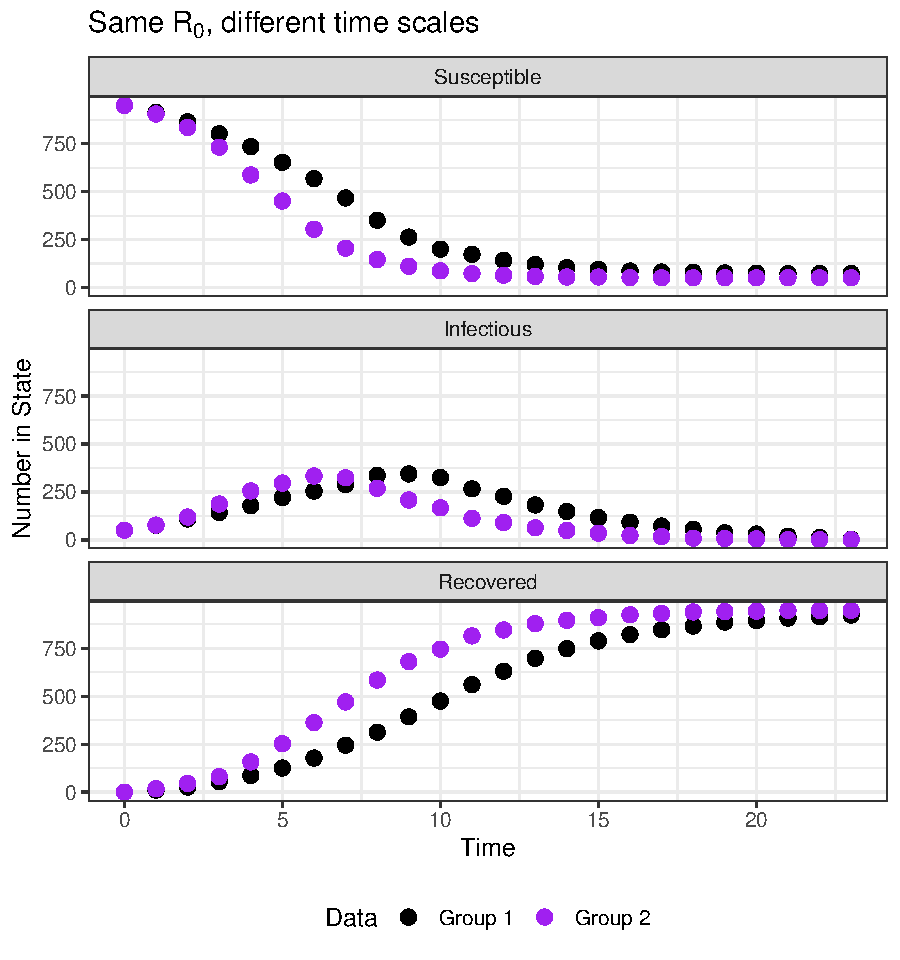
\includegraphics[width = .5\textwidth]{images/diff-time-standard.pdf}%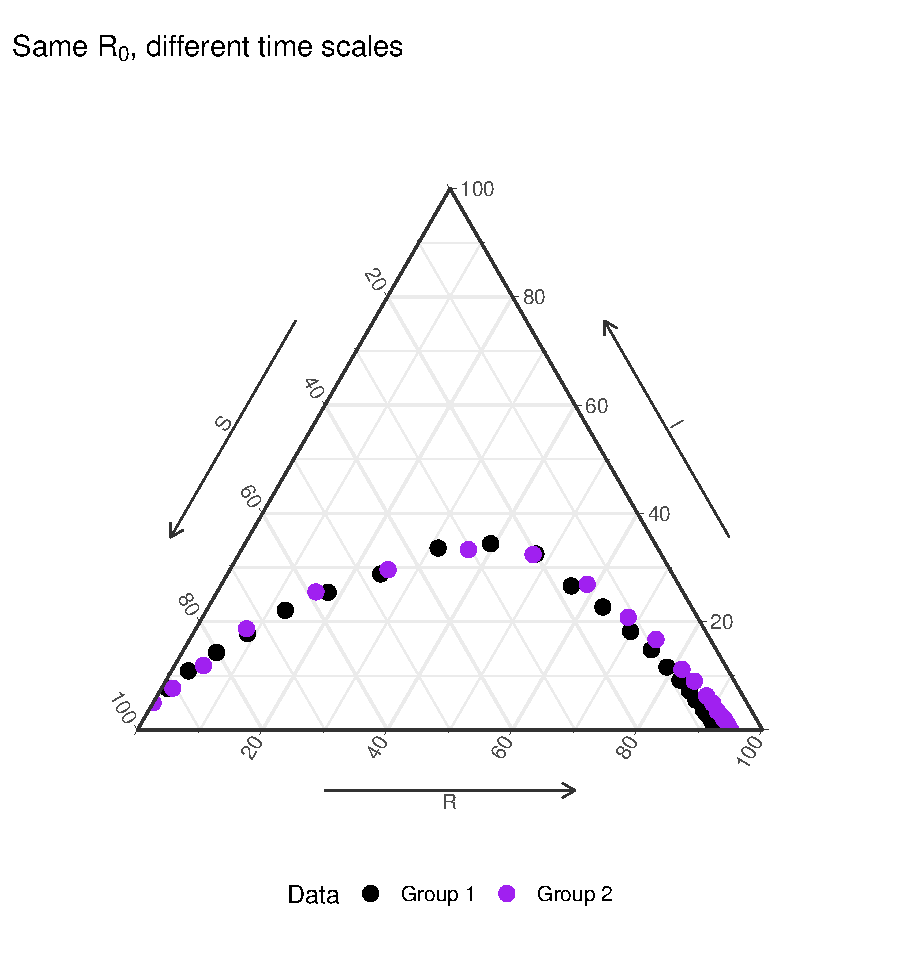
\includegraphics[width = .5\textwidth]{images/diff-time-ternary.pdf}
    \caption{Bivariate view of \# in each state vs. time. Both data sets are generated using the same value of $R_0 = 2.8$ but have different values of $\beta$ and $\gamma$.\textcolor{violet}{We probably need to define $\beta/\gamma$.}
\textcolor{violet}{NEW: recommendation - make this plot actually have 3 examples (the current one), one where we have an affine transformation of the time scale, and one with the halleolof data.} \textcolor{violet}{Also these figures should be reproducible.}}
    \label{fig:different-scales-standard}
\end{figure}

\subsection[ternary visualizations]{Ternary and time-invariant
visualizations for \(R_0\)}\label{sec:ternary}

It is possible to identify, at a glance, which SIR epidemic paths, like
those in Fig. \ref{fig:different-scales-tern} have the same value of
\(R_0\) via ``time-invariant'' visualizations, under some circumstances.
Specifically, for SIR models we propose using ternary to examine an
epidemic's trajectory in a more time-invariant manner.

Ternary plots are sometimes used in chemistry \citep[][]{Gillespie1976}
but only rarely seen in the field of infectious disease epidemiology (to
our knowledge, only seen in \cite{}). Ternary plots illustrate the
relationship of constrained 3D data, namely of points
\((a_i, b_i, c_i) \in [0,1] \times [0,1] \times [0,1]\) with
\(a_i+ b_i + c_i =1\) and as such, are situational. The SIR framework
happens to be of the situational format required for ternary plots where
\((S(t), I(t), R(t))\) are the number of susceptible, infectious, and
recovered individuals in each state at time \(t\) and
\(S(t) + I(t) + R(t) = N(t)\) where \(N(t)\) is the population size at
time \(t\).

Ternary plots are time-invariant in the sense that the temporal scale
does not explicitly apear in the visualization and as a consequence,
allow for direct comparisons of outbreaks on different time scales
(e.g.~days vs.~years) or of SIR data of the same disease in different
areas (our first case study in Sec. \ref{sec:ex1} focuses on this).

To show that ternary plots have to potential to aid in the comparison of
different epidemic's \(R_0\)s -in certain circumstances- we first need
to introduce the classic, deterministic Kermack and McKendrick
\cite{CITETHIS?} SIR model where the initial number in each state
\((S(0), I(0), R(0))\) are known and \(N\) the population size is
constant. The movement of individuals among the states is given by the
following differential equations (Eq. \eqref{eq:sir-ode}) where
\(\beta\) is the average infection rate and \(\gamma\) is the average
recovery rate, \begin{align}\label{eq:sir-ode}
      S^\prime(t) &= -\frac{\beta S(t)I(t)}{N} \\
      I^\prime(t) &= \frac{\beta S(t)I(t)}{N} - \gamma I(t) \nonumber\\
      R^\prime(t) &= \gamma I(t) \nonumber.
  \end{align}

\textcolor{violet}{SUGGESTION: define $R_0$ mathematically here (though referred to in figure 2 - which still needs to be defined there).}

If we have two SIR models that follow the Kermack and McKendrick SIR
model, have the same percentage of individuals in the initial states,
and the same value of \(R_0\) then the two models will create exactly
overlapping paths in a ternary plot.

More formally, let two Kermack and McKendrick (see Eq.
\eqref{eq:sir-ode}) SIR models be denoted \((S_1(t), I_1(t), R_1(t))\)
and \((S_2(t), I_2(t), R_2(t))\), respectively, for \(t > 0\). Assume
both models have initial values \((S(0), I(0), R(0))\). Let
\(R_0 = \frac{\beta_1}{\gamma_1} = \frac{\beta_2}{\gamma_2}\) where
\(\beta_i\) and \(\gamma_i\) are the average infection rate and recovery
rate, respectively, for SIR model \(i=1, 2\). Equivalently,
\(\beta_2 = a \beta_1\) if and only if \(\gamma_2 = a \gamma_1\) for
some \(a > 0\).

\begin{theorem}\label{thm:sir-scale}
Let there be two SIR models as described above.  Then for all $t > 0$ there exists an $s$ such that $(S_1(t), I_1(t), R_1(t)) = (S_2(s), I_2(s), R_2(s))$.  Moreover, $s = \frac{1}{a}t$.
\end{theorem}

The proof of Theorem \ref{thm:sir-scale} relies on a fairly recent
result from \cite{Harko2014} and is shown in detail in Appendix
\ref{app:proof}. The consequence of Theorem \ref{thm:sir-scale} is that
for two SIR models that have the same initial percent of individuals in
each state and \(R_0\) then for every point on the epidemic path of the
first SIR model is also a point on the epidemic path of the second SIR
model. Taking the sample simulations from Fig.
\ref{fig:different-scales-standard}, Fig.
\ref{fig:different-scales-tern} presents these models in a ternary plot.

\begin{figure}[!ht]
%% Code to reproduce is in inst/paper_figs/different-time-scales.R
    \centering
    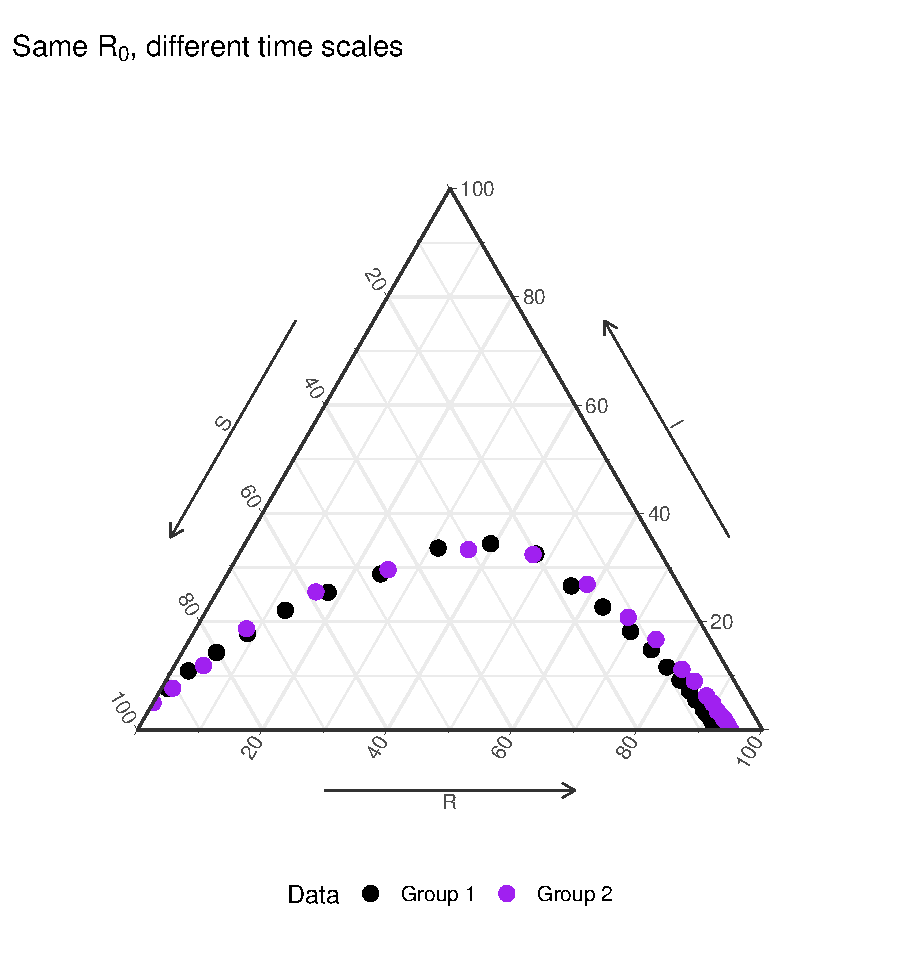
\includegraphics[width = .5\textwidth]{images/diff-time-ternary.pdf}
    \caption{Ternary view of \# in each state.  Both this Fig. and Fig. \ref{fig:different-scales-standard} display the same two sets of data.  Both data sets are generated using the same value of $R_0 = 2.8$ but have different values of $\beta$ and $\gamma$. \textcolor{violet}{We probably need to define $\beta/\gamma$.}  While there are obvious are differences in Fig.\ref{fig:different-scale-standard}, the data sets look quite similar in the ternary view. \textcolor{violet}{I might suggest using opacity to show time scale here?} \textcolor{violet}{Make this reproducible too?}}
    \label{fig:different-scales-tern}
\end{figure}

In \pkg{EpiCompare}, we also provide visualization tools to aid in
comparing models in the ternary / time-invariant space, which is
presented in more details in Section
\ref{sec:time-invariant-in-simplex}.

\subsection[Simplexes beyond ternary plots]{Simplexes beyond ternary
plots and time-invariant comparison
tools}\label{sec:time-invariant-in-simplex}

Beyond ternary plots, and the associated SIR models, we can extend the
time-invariant approach described in Section \ref{sec:ternary} to higher
dimensions (i.e.~models with more states). The constraints in 3d that
are met with the SIR model (that is
\(\sum_{i=1}^3 (\text{number in state}(i)) = N(t)\)) actually represents
a spaces of 3d simplexes, and the ternary plot specifically represents
these after scaling to examine such values as proportions (ternary plots
are known as a 3d unit simplex due to it's scaling). This same scaling
for larger models (i.e.~with more states) can be done onto different
simplexes. In this package we present tools to help compare models
(mostly through similations), and this tool compares these objects after
projecting them into a one-dimension less space through the simplexical
structure of the data.

In \pkg{EpiCompare} we allow for the compare epidemics in these higher
dimensional spaces by first projecting onto these simplexes. Even though
higher dimensional models may not be able to visualized, we provide
multiple tools to aid in the comparison of models and epidemics. The
first of which uses multiple simulations under specific model parameters
to assess the bairabilty of the model fit. In \pkg{EpiCompare} we
provide ways to create prediction regions for a true epidemic under the
model assumptions using these simulations. These regions require
representing multi-dimensional structures for functions to completely
contain epidemics, and treat these simulations and epidmeics as
filamental objects. We extend off of papers like \citet{Dalmasso2019a}
to create these bands. These high dimensional bands allow the user to
assess if the true epidemic is within the band (there-by assessing the
model's representation of the epidemic), and also compare who different
models are from each other through distances that compare sets. We
recommend using the Hausdorff distance to compare such sets as it
captures how much bigger the sets would have to expand to cover each
other, and is defined mathematically as \[
d_\text{Hausdorff}(S_1, S_2) = \max \left\{ \sup_{x \in S_1} \inf_{y \in S_2} d(x,y) \;,\; \sup_{y \in S_2} \inf_{x \in S_1} d(x,y)\right\}\;.
\]

\section[Package overview]{Package tool overview}\label{sec:overview}

\hypertarget{rmd-code-formatting-info}{%
\subsection{RMD Code formatting info}\label{rmd-code-formatting-info}}

This is the Section \ref{sec:intro}. This template demonstrates some of
the basic LaTeX that you need to know to create a JSS article.

In general, don't use Markdown, but use the more precise LaTeX commands
instead:

\begin{itemize}
\item
  \proglang{Java}
\item
  \pkg{plyr}
\end{itemize}

One exception is inline code, which can be written inside a pair of
backticks (i.e., using the Markdown syntax).

If you want to use LaTeX commands in headers, you need to provide a
\texttt{short-title} attribute. You can also provide a custom identifier
if necessary. See the header of Section \ref{r-code} for example.

\subsection[R code]{RMD \proglang{R} code}\label{r-code}

Can be inserted in regular R markdown blocks.

hags hags hags \cite{Neal2004}

\begin{CodeChunk}
\begin{CodeInput}
R> x <- 1:10
R> x
\end{CodeInput}
\begin{CodeOutput}
 [1]  1  2  3  4  5  6  7  8  9 10
\end{CodeOutput}
\end{CodeChunk}

\section[Tour]{A tour of \pkg{EpiCompare}}\label{sec:tour}

In this section, we highlight a number of the functionalities available
in \proglang{EpiCompare}. These functionalities include data cleaning,
visualization, simulation, and comparison, in accordance with the data
analysis pipeline REF\ref{}. We show a full data analysis from beginning
to end that can be accomplished in a streamlined and standardized
manner.

\subsection{Data and exploratory analysis}

We analyze an outbreak of measles in the town of Hagelloch, Germany from
1861-1862, a data set organized by \cite{pfeilsticker1863}. The data was
later made visible by \cite{oesterle1992} and made available in an
\proglang{R} by \cite{surveillance2017}. The Hagelloch data includes a
rich set of features including household members, school level,
household locations, date of first symptoms (prodromes), date of measles
rash, and even the alleged infector. A subset of the data is shown in
Table \ref{tab:hags-people}. Because of these rich features, this data
set has been an ideal testing ground methodology in infectious disease
epidemiology and is used in work by
\cite{Neal2004,britton2011,groendyke2012,becker2016}.

\begin{CodeChunk}
\begin{table}[!h]

\caption{\label{tab:hags-people}Subset of Hagelloch infection data.  Features include the person ID, household ID (HH ID), age, sex, class level (Pre-K/1st/2nd), date of first symptoms, date of the appearance of the measles rash, and the alleged infector ID of the individual.}
\centering
\begin{tabular}[t]{rrlrllllr}
\toprule
ID & HH ID & Name & Age & Sex & Class & Symp. Start & Rash Date & Infector ID\\
\midrule
1 & 61 & Mueller & 7 & female & 1st class & 1861-11-21 & 1861-11-25 & 45\\
2 & 61 & Mueller & 6 & female & 1st class & 1861-11-23 & 1861-11-27 & 45\\
3 & 61 & Mueller & 4 & female & preschool & 1861-11-28 & 1861-12-02 & 172\\
4 & 62 & Seibold & 13 & male & 2nd class & 1861-11-27 & 1861-11-28 & 180\\
5 & 63 & Motzer & 8 & female & 1st class & 1861-11-22 & 1861-11-27 & 45\\
45 & 51 & Goehring & 7 & male & 1st class & 1861-11-11 & 1861-11-13 & 184\\
\bottomrule
\end{tabular}
\end{table}

\end{CodeChunk}

With \pkg{EpiCompare}, we can easily obtain the empirical cumulative
incidence function with respect to the measles rash appearance (variable
\code{ERU}) with the following tidy-style function,
\code{agents_to_aggregate}. The function \code{agents_to_aggregate} is a
key component of \pkg{EpiCompare}, allowing the user to easily switch
from an individual-level (i.e.~an agent) view of a disease to an
aggregate level. For example, the below code shows how we can convert
the agent data to a cumulative incidence of the measles rash, in order
to see how the disease spread through the population over time. We can
then compare the cumulative incidence of the rash to the cumulative
incidence of the prodromes, i.e.~the initial symptoms. We do this with
the below code, and a part of the cumulative incidence data output are
shown in Table \ref{tab:cif-rash}. The argument
\code{integer_time_expansion} indicates whether we should include all
time points in the recorded range of the data or only when there is a
change in the incidence.

\begin{CodeChunk}
\begin{CodeInput}
R> cif_rash  <- hagelloch_raw %>%
+   mutate(time_of_rash = as.numeric(ERU - min(PRO, na.rm = TRUE))) %>%
+   agents_to_aggregate(states = time_of_rash,
+                       integer_time_expansion = FALSE) %>%
+   mutate(type = "Rash")
\end{CodeInput}
\end{CodeChunk}

\begin{CodeChunk}
\begin{table}[!h]

\caption{\label{tab:cif-rash}Turning the individual-level information from the Hagelloch data to an aggregate view of the cumulative incidence of the measles rash in the population over time.}
\centering
\begin{tabular}[t]{rrr}
\toprule
Time & \# Susceptible & \# Total rash appearances\\
\midrule
0 & 188 & 0\\
4 & 187 & 1\\
7 & 186 & 2\\
9 & 185 & 3\\
12 & 183 & 5\\
\bottomrule
\end{tabular}
\end{table}

\end{CodeChunk}

One question of interest is the duration between initial onset of
prodromes or symptoms and the appearance of the measles rash. Since
\code{agent_to_aggregate} outputs a tidy-style data frame, it is a
simple task to plot the two sets of incidence curves on the same graph
(Fig. \ref{fig:cifs}).

\begin{CodeChunk}
\begin{CodeInput}
R> cif_prodromes <- hagelloch_raw %>%
+   mutate(time_of_PRO = as.numeric(PRO - min(PRO, na.rm = TRUE))) %>%
+   agents_to_aggregate(states = time_of_PRO,
+                       integer_time_expansion = FALSE) %>%
+   mutate(type = "Pro")
\end{CodeInput}
\end{CodeChunk}

\begin{CodeChunk}
\begin{CodeInput}
R> plot_df <- bind_rows(cif_rash, cif_prodromes)
R> 
R> ggplot(data = plot_df,
+        aes(x = t, y = X1, col = type)) + 
+   geom_step() + 
+   labs(title = "Cumulative incidence of measles appearance",
+        x = "Time (days relative to first prodrome appearance)",
+        y = "Cumulative incidence of event") + 
+   coord_cartesian(xlim = c(0, 55)) +
+   scale_color_manual(values = c("blue", "red"))
\end{CodeInput}
\begin{figure}[H]

{\centering 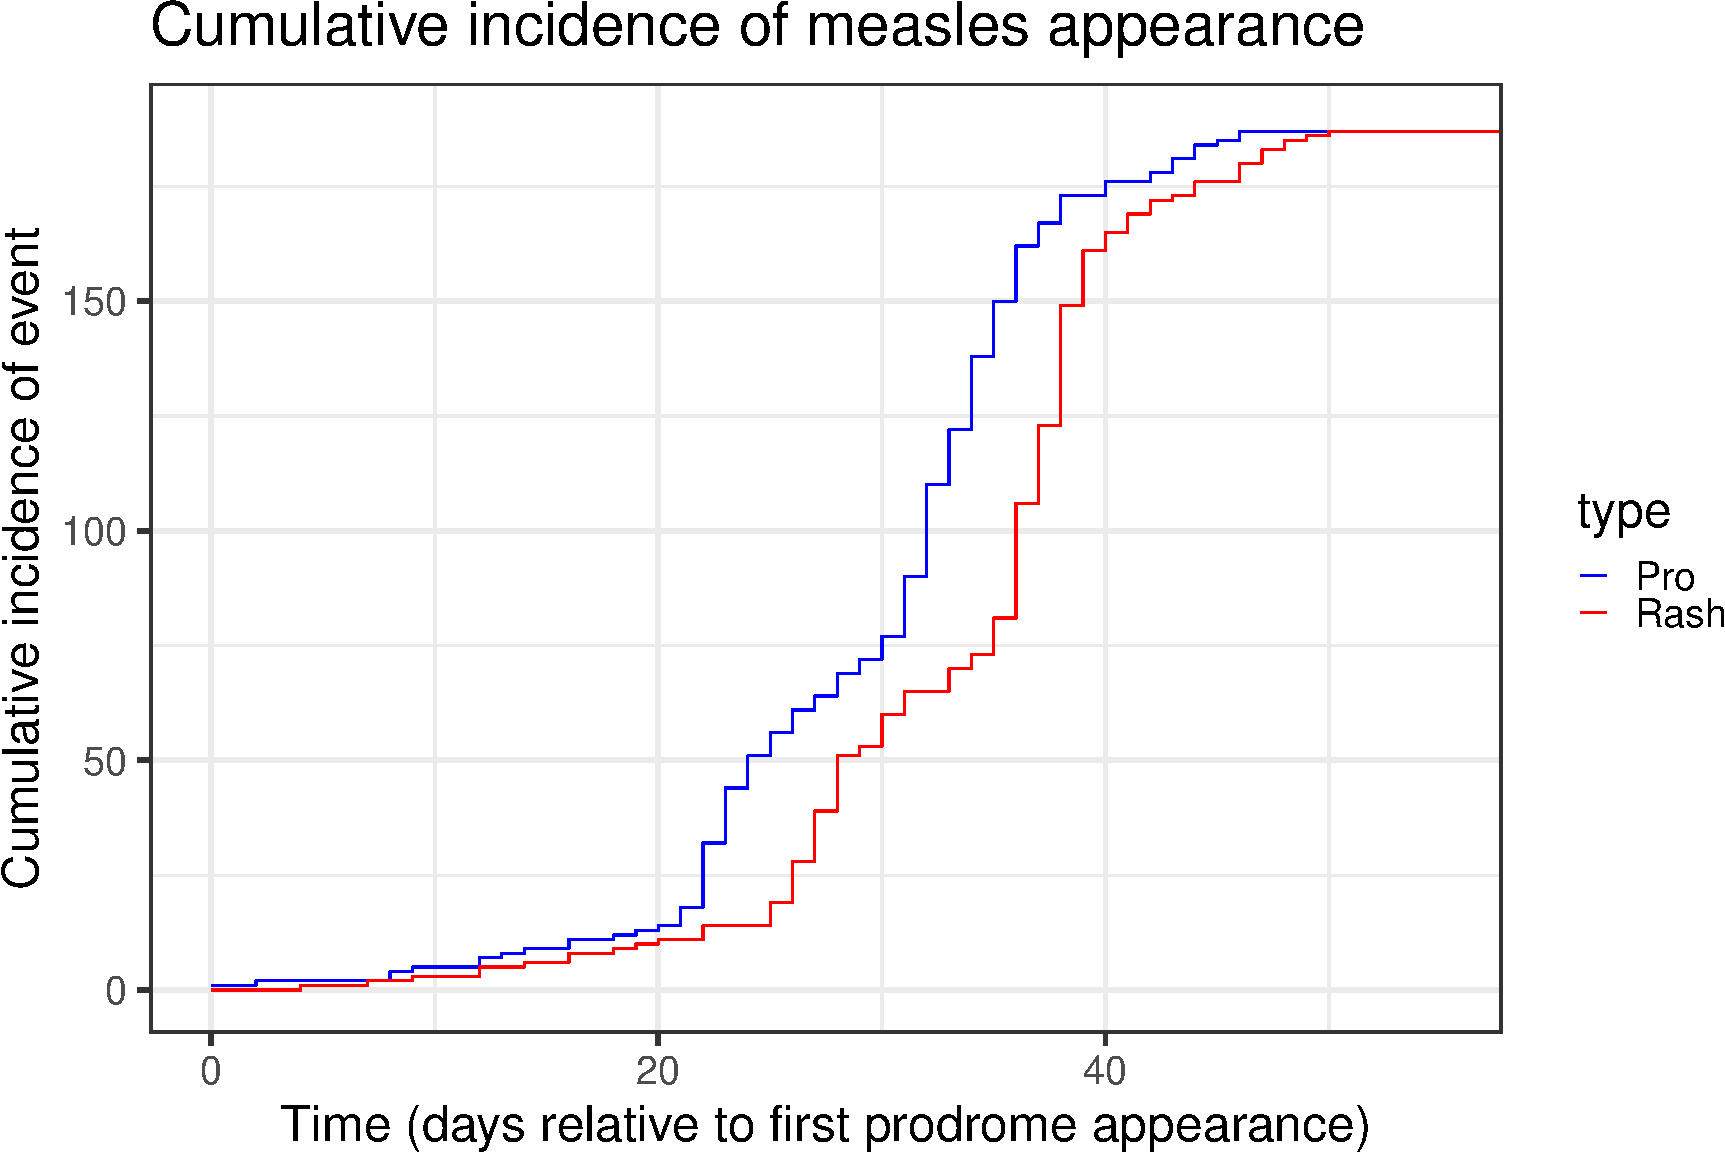
\includegraphics{Figs/unnamed-chunk-6-1} 

}

\caption{\label{fig:cifs}Empirical cumulative incidence functions of prodrome (symptom) onset and measles rash appearance.  We see that there is approximately a a constant lag between the two curves.}\label{fig:unnamed-chunk-6}
\end{figure}
\end{CodeChunk}

The real power of \code{agents_to_aggregate()} lies in its ability to
aggregate over any number of pre-specified states. For example, the
Hagelloch data sets contains two columns, \code{tI} and \code{tR}, the
time of infection and recovery, respectively of each individual. We can
then plot the SIR values through a time-invariant lens using
\pkg{ggplot2} and \pkg{ggtern} functions (as shown in Fig.
\ref{fig:hag-tern-raw}) or with our custom \code{geom},
\code{geom_aggregate}, which takes the raw agent data as input.

\begin{CodeChunk}
\begin{CodeInput}
R> hagelloch_sir <- hagelloch_raw %>%
+   agents_to_aggregate(states = c(tI, tR),
+                       min_max_time = c(0, 55)) %>%
+   rename(time = t, S = X0, I = X1, R = X2)
R> 
R> 
R> ggplot(hagelloch_sir, aes(x = S, y = I, z = R))+
+   coord_tern() +
+   geom_path() +
+   labs(x = "S", y = "I", z = "R",
+        title = "Time invariant view of Hagelloch measles outbreak") + 
+   theme_sir(base_size = 24)
\end{CodeInput}
\begin{figure}[H]

{\centering 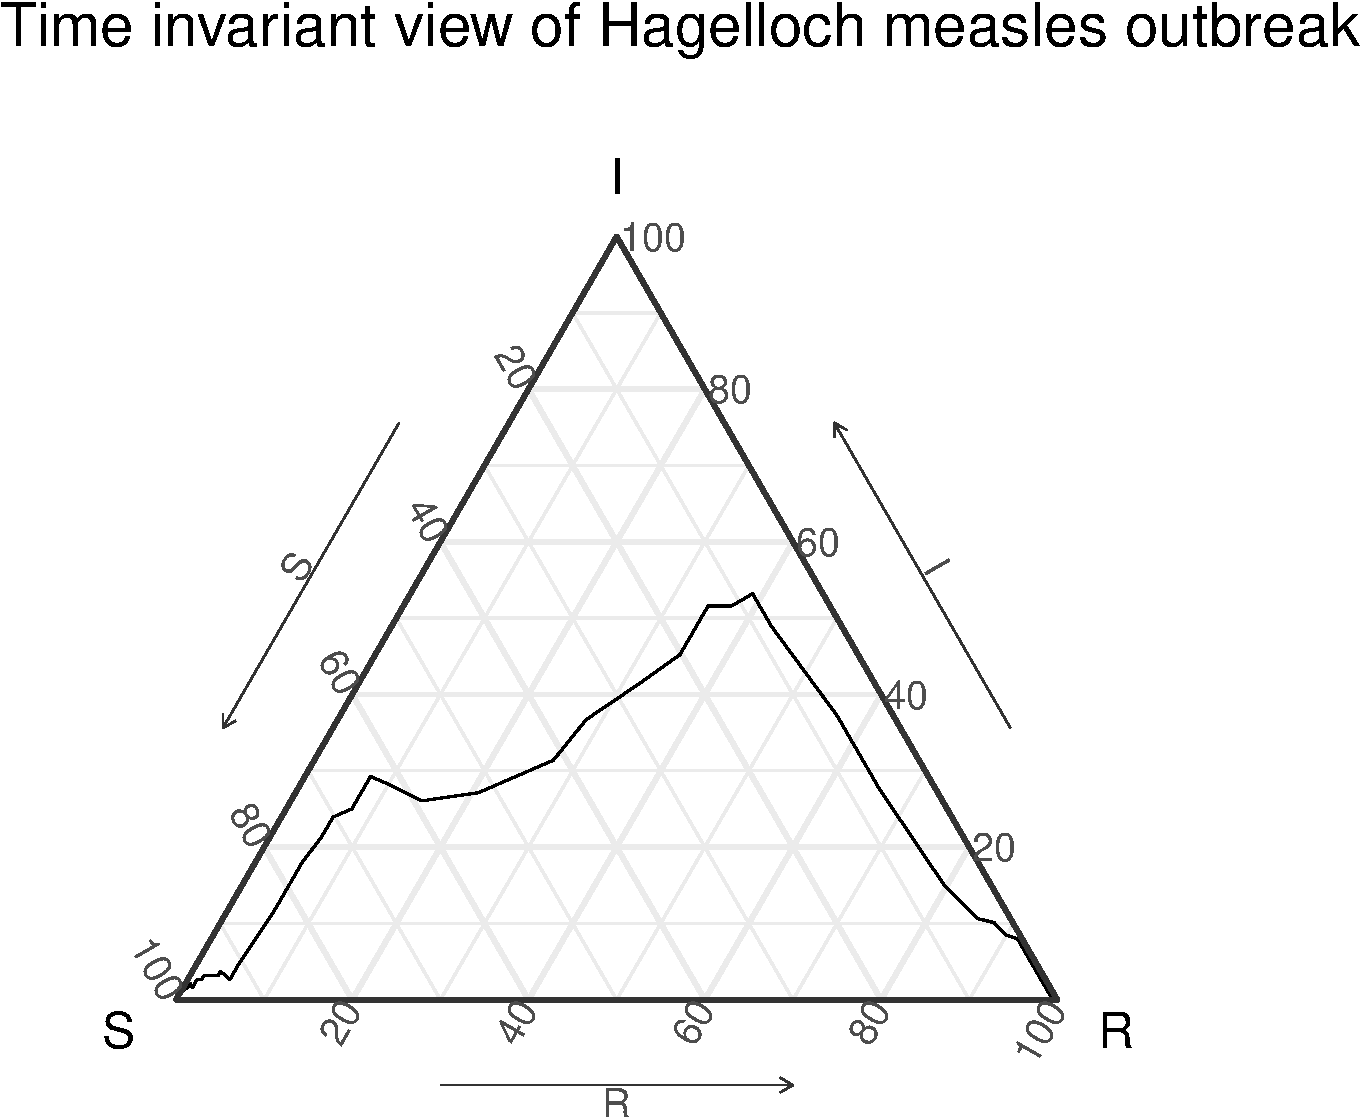
\includegraphics{Figs/unnamed-chunk-8-1} 

}

\caption{\label{fig:hag-tern-raw}Time invariant view of the Hagelloch epidemic where we view the individuals in Susceptible, Infectious, or Recovered states.  We see there are two peaks of infection (the vertical axis).}\label{fig:unnamed-chunk-8}
\end{figure}
\end{CodeChunk}

Moreover, we can look at the outbreaks of the disease by group within
\code{agent_to_aggregate()} or \code{geom_aggregate()}. This allows us
to examine differences among the different groups of individuals. For
example, we show the time invariant outbreak by class level in Figure
\ref{fig:tern-class-data}. Immediately, we see that time invariant
infection curve is different for the pre-school class compared to the
1st class. In the 1st class, we see about 95\% of the class become
infected and less than 10\% of them having recovered, which is
indicative of a super-spreading event. This suspicion is further
confirmed in that 26 of the 30 1st class students have been reportedly
infected by the same individual.

\begin{CodeChunk}
\begin{CodeInput}
R> hagelloch_raw %>%
+   ggplot(aes(y = tI, z = tR, color = CL)) +
+   geom_aggregate(size = 2) + coord_tern() +
+   labs(x = "S", y = "I", z = "R",
+        color = "Class") +
+   scale_color_brewer(palette = "Dark2") +
+   facet_wrap(~CL)
\end{CodeInput}
\begin{figure}[H]

{\centering 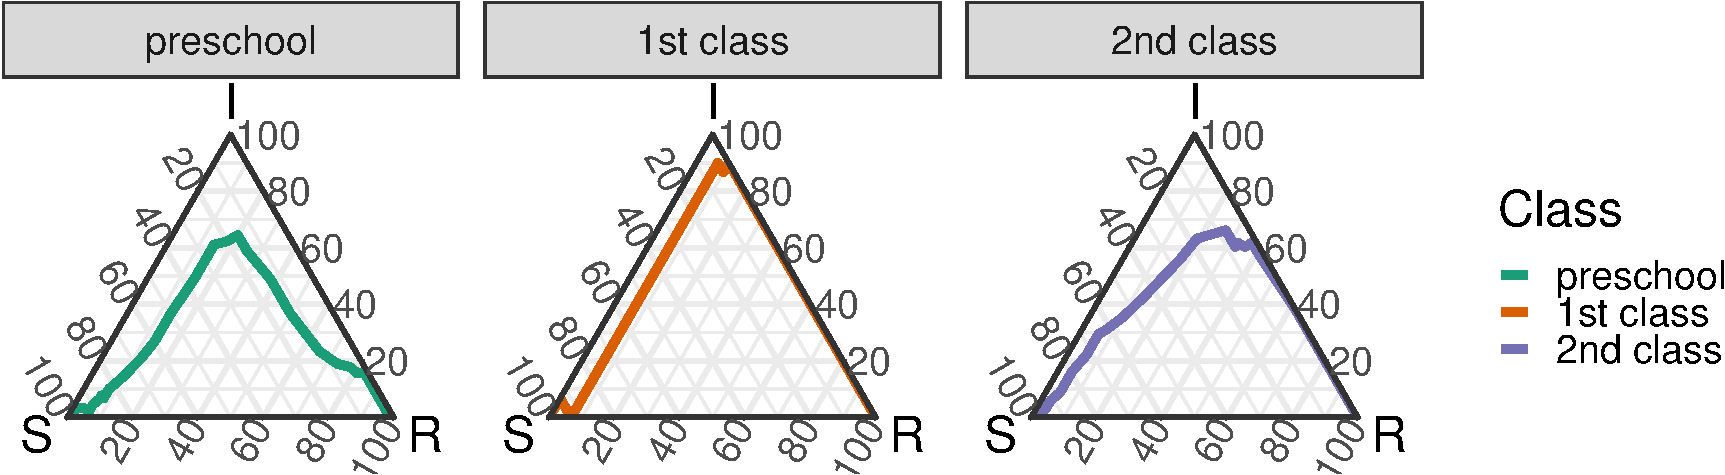
\includegraphics{Figs/unnamed-chunk-9-1} 

}

\caption{\label{fig:tern-class-data}Time invariant outbreak curves for the three class groups.  The pre-school class has a distinct peak of infection whereas the peak infection point for the other two classes are less well defined.}\label{fig:unnamed-chunk-9}
\end{figure}
\end{CodeChunk}

Along with multiple epidemic states, the function
\code{agents_to_aggregate} can also be extended to populations with
vital dynamics (e.g.~birth and death) and examples of this are shown in
the package vignette. In summary, \code{agents_to_aggregate()} is a
multi-purpose workhorse that may be leveraged to convert individual
level records into aggregate information that may be more useful for
some forms of epidemic modeling such as compartment modeling.

Up to this point, we have used \pkg{EpiCompare} in the context of
observed data. We also want to compare statistical models, and
\pkg{EpiCompare} aids in that process via a simple but dynamic
individual-level data generator, conversion tools for popular epidemic
model packages, and model assessments. We demonstrate an example here.

We first try to model the Hagelloch data with an SIR model (see Eq.
\ref{eq:sir}). In our vignette, we show how to fit a stochastic model
via maximum likelihood and simulate from the model with those best fit
parameters. Our function \code{simulate_agents()} generates individual
level data according to discrete multinomial draws, which depend on the
number of individuals in each state at the previous time step and a
matrix of transition probabilities. For example, the below code
generates 100 simulations of an outbreak of a diseease with one initial
infector in a population of \(n= 188\) individuals.

\begin{CodeChunk}
\begin{CodeInput}
R> trans_mat <- matrix(c("X0 * (1 - X1 * par1 / N)", "X0 * X1  * par1 / N", "0",
+                   "0", "X1 * (1 - par2)", "par2 * X1",
+                   "0", "0", "X2"), byrow = TRUE, nrow = 3)
\end{CodeInput}
\end{CodeChunk}

\begin{CodeChunk}
\begin{CodeInput}
R> set.seed(2020)
R> 
R> best_params <- c("beta" = .36, "gamma" = .13)
R> ## This is the SIR representation
R> 
R> rownames(trans_mat) <- c("S", "I", "R")
R> init_vals <- c(187, 1, 0)
R> par_vals <- c(par1 = best_params[1], par2 = best_params[2])
R> max_T <- 55
R> n_sims <- 100
R> 
R> agents <- simulate_agents(trans_mat,
+                        init_vals,
+                        par_vals,
+                        max_T,
+                        n_sims,
+                        verbose = FALSE)
\end{CodeInput}
\end{CodeChunk}

\begin{CodeChunk}
\begin{CodeInput}
R> agg_model <- agents %>% group_by(sim) %>%
+   agents_to_aggregate(states = c(I, R)) %>%
+   mutate(Type = "Simple SIR")
\end{CodeInput}
\end{CodeChunk}

The result of our simulation is the object \code{agents} which is a
18800 \(\times\) 5 which details the time of entry into the \(S\),
\(I\), and \(R\) states for a given simulation. Before we examine the
results of this simple SIR model, we will also examine another, more
sophisticated SIR model, this time from the package \pkg{EpiModel}.
Briefly, this model first fits a contact network to the set of
indivduals, where the class of the student is a covariate. The model
then simulates a SIR-epidemic on that network.

\begin{CodeChunk}
\begin{CodeInput}
R> library(EpiModel)
R> ## WARNING:  Will take a minute or two
R> 
R> set.seed(42)
R> nw <- network.initialize(n = 188, directed = FALSE)
R> nw <- set.vertex.attribute(nw, "group", rep(0:2, each = 90, 30, 68))
R> formation <- ~edges + nodematch("group") + concurrent
R> target.stats <- c(200, 300, 200)
R> coef.diss <- dissolution_coefs(dissolution = ~offset(edges),  duration = 5)
R> est1 <- netest(nw, formation, target.stats, coef.diss, edapprox = TRUE)
R> 
R> param <- param.net(inf.prob = 0.1, act.rate = 5, rec.rate = 0.1)
R> status.vector <- c(rep(0, 90), rep(0, 30), rep(0, 67), 1)
R> status.vector <- ifelse(status.vector == 1, "i", "s")
R> init <- init.net(status.vector = status.vector)
R> control <- control.net(type = "SIR", nsteps = 55,
+                        nsims = 100, epi.by = "group")
R> epimodel_sir <- netsim(est1, param, init, control)
\end{CodeInput}
\end{CodeChunk}

The output of this model is \code{epimodel_sir}, an object of class
netsim, which contains a plethora of modeling information. We provide
the function \code{fortify_aggregate()}, which can take objects from
specialized classes of modeling output and transform it into a
tidy-style data frame.

\begin{CodeChunk}
\begin{CodeInput}
R> fortified_net <- fortify_aggregate(epimodel_sir, 
+                                    states = c("s.num", "i.num", "r.num")) %>%
+   mutate(Type = "EpiModel SIR",
+          sim = as.numeric(gsub("sim", "", sim)))
\end{CodeInput}
\end{CodeChunk}

We can then analyze the results of the two models side by side as
time-invariant epidemic curves. The results are shown in Figure
\ref{fig:hag-simple-sir}, where a 90\% prediction band is estimated from
the delta ball method for each of the two models. For the Simple SIR
model, we see that the data generally covers the data fairly well but
clearly misses the second peak of infection. We also see that the
prediction band is very large, covering up a large area of the ternary
plot. On the other hand, for the \pkg{EpiModel} model, we see that the
prediction band covers the data quite well and takes up less area.

\begin{CodeChunk}
\begin{CodeInput}
R> both_models <- bind_rows(agg_model, fortified_net)
R> 
R> 
R> g <- ggplot() + geom_prediction_band(data = both_models %>% filter(t != 0),
+          aes(x = X0, y = X1, z = X2,
+               sim_group = sim, fill = Type),
+          alpha = .5,
+          conf_level = .90) 
\end{CodeInput}
\end{CodeChunk}

\begin{CodeChunk}
\begin{CodeInput}
R> g +   geom_path(data = both_models %>% filter(t !=0),
+             aes(x = X0, y = X1, z = X2, group = paste(Type, sim)),
+             alpha = .3, col = "gray40") + 
+     coord_tern() + theme_sir(base_size = 24) +
+   geom_point(data = hagelloch_sir,
+              aes(x = S, y = I, z =R), col = "black") +
+   labs(title = "Simple SIR model",
+        subtitle = "90% Prediction band and original data",
+        x = "S", y = "I", z = "R") +
+   scale_fill_manual(values = c("#006677", "#AA6600")) + 
+   facet_wrap(~Type) +
+   theme(legend.position = "bottom")
\end{CodeInput}
\begin{figure}[H]

{\centering 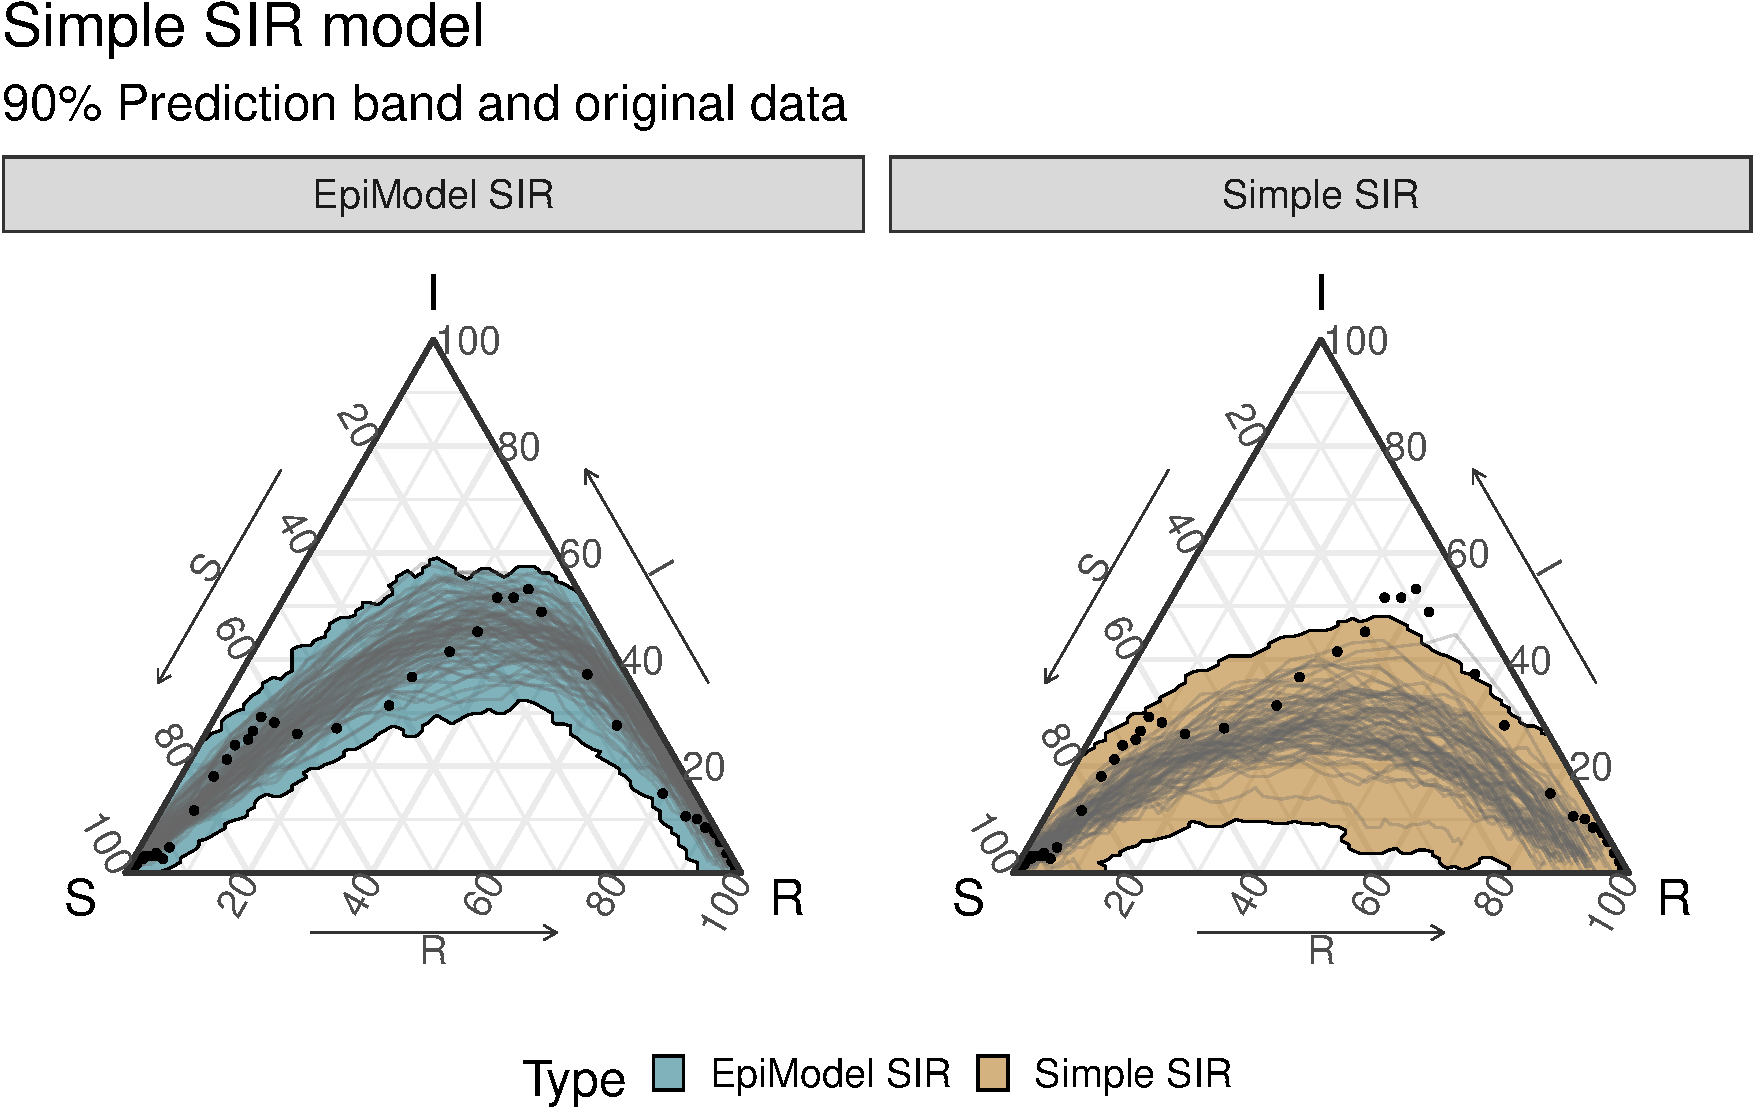
\includegraphics{Figs/unnamed-chunk-16-1} 

}

\caption{\label{fig:hag-simple-sir}  Original Hagelloch SIR data (black) along with 90\% prediction band and actual simulation paths from the Simple SIR and the EpiModel SIR models.}\label{fig:unnamed-chunk-16}
\end{figure}
\end{CodeChunk}

However, both models are not a good fit to the filamental path as
opposed to the individual points in \((S, I, R)\)-space. This can be
captures with the set of simulations both models predict, which all
generally have a single defined peak of infection whereas the data
certainly looks like it has two distinct peaks, likely caused by our
assumed super-spreader event. This observation is backed up by the below
analysis that demonstrates that the estimated psuedo-density of the
observed epidemic (relative to the simulations from either model) is
much less likely then \textbf{any} of the simulations (reported in Table
\ref{tab:hags-extreme}. In conclusion, \pkg{EpiCompare} makes it clear
that, at a glance, 1) the EpiModel network model is a better fit than
the Simple SIR model, and 2) the fit is only good at the individual
point level as opposed to the epidemic path level.

\begin{CodeChunk}
\begin{CodeInput}
R> #-- after cleaning up and combining --
R> all_together_df <- rbind(simple_sir,
+                          hagelloch_sir2)
\end{CodeInput}
\end{CodeChunk}

\begin{CodeChunk}
\begin{table}[!h]

\caption{\label{tab:cif-all-together-df}Top and bottom 2 rows of \tt{all\_together\_df}\text{, combining both simulated epidemics and the true epidemic.}}
\centering
\begin{tabular}[t]{lrrrrr}
\toprule
Type & sim & t & S & I & R\\
\midrule
Simple SIR & 1 & 0 & 188 & 0 & 0\\
Simple SIR & 1 & 1 & 187 & 1 & 0\\
true observation & 0 & 54 & 1 & 0 & 187\\
true observation & 0 & 55 & 1 & 0 & 187\\
\bottomrule
\end{tabular}
\end{table}

\end{CodeChunk}

\begin{CodeChunk}
\begin{CodeInput}
R> compression_df <- all_together_df %>% group_by(Type, sim) %>% 
+   filament_compression(data_columns = c("S","I","R"), 
+                        number_points = 20)
\end{CodeInput}
\end{CodeChunk}

\begin{CodeChunk}
\begin{CodeInput}
R> dmat <- compression_df %>% 
+   dist_matrix_innersq_direction(
+     position = c(1:length(compression_df))[
+       names(compression_df) %in% c("S","I", "R")],
+     id_as_columns = T)
R> 
R> tdmat <- tidy_dist_mat(as.matrix(dmat[,-c(1:2)]),
+                        rownames_df = ungroup(dmat[,1:2]),
+                        colnames_df = ungroup(dmat[,1:2])) 
R> 
R> 
R> simple_sir_true_obs_info <- tdmat %>% 
+   compare_new_to_rest_via_distance(
+     new_name_id = data.frame(Type = "true observation", sim = 0),
+     distance_func = distance_psuedo_density_function, 
+     sigma = "20%") 
\end{CodeInput}
\end{CodeChunk}

\begin{CodeChunk}
\begin{table}[!h]

\caption{\label{tab:hags-extreme}The extremeness of the true simulations based on comparing psuedo-density estimates between true vs simulated curves}
\centering
\begin{tabular}[t]{l>{\raggedleft\arraybackslash}p{6cm}>{\raggedleft\arraybackslash}p{6cm}}
\toprule
Type & simulations-based estimated psuedo-density & proportion of simulations with lower estimated psuedo-density\\
\midrule
Simple SIR & 0.0036733 & 0\\
EpiModel SIR & 0.0028813 & 0\\
\bottomrule
\end{tabular}
\end{table}

\end{CodeChunk}

\bibliography{EpiCompare.bib}


\end{document}

